\documentclass[14pt]{beamer}
\usepackage[utf8]{inputenc}
\usepackage{graphicx}
\usepackage{listings}
\usepackage{helvet}
%\usetheme{Singapore}

% FrameNr 
%\setbeamertemplate{footline}{%
%\begin{beamercolorbox}[wd=\paperwidth,ht=2.25ex,dp=1ex]{date in head/foot}%
%\hspace*{1ex} \insertframenumber{} / \inserttotalframenumber
%\hspace*{35ex}titlename
%\end{beamercolorbox}}%

\title{Skulls - coreboot your X230 the easy way}
\author{Martin Kepplinger}

\begin{document}

\begin{frame}
\titlepage
%\includegraphics[width=40pt]{logo}
%/Documentation/logo.gif
\end{frame}

%\begin{frame}
%\frametitle{toc}
%\tableofcontents
%\end{frame}

\begin{frame}
Who am I?

- work for https://www.ginzinger.com/en/ in Austria

- kernel developer, C programming, tslib maintainer, ...

- use Tor!
\end{frame}


\begin{frame}
Let's curl an image and coreboot your Laptop!
\end{frame}

\begin{frame}
Lenovo Thinkpad X230 Laptop
\end{frame}


\begin{frame}
3rd gen. Intel i series (Ivy Bridge)

%one of the more performant Laptops supported by coreboot

%still, from 2012
\end{frame}


\begin{frame}
The coreboot project
\end{frame}


\begin{frame}
https://coreboot.org - "for end users"

"coreboot is a replacement for your BIOS / UEFI with a strong focus on boot speed, security and flexibility."

free software (GPL)

hardware init / ACPI interface
\end{frame}

\begin{frame}
coreboot distributions
\end{frame}


\begin{frame}
it's all there, but how to configure and how to flash
(how to or not to enable internal flashing without disassembling)
\pause

- Libreboot (X200)

- Heads (X230, Librem Laptops)

- Skulls - not quite Heads (X230)

They all release binary flash image files
%or offer to build them reproducibly
\end{frame}


\begin{frame}
Skulls goals
\end{frame}


\begin{frame}
\texttt{
faadfce initial infos
}
\texttt{
 75b154334d.config | 686 ++++++++++++++++++++++++++++++++++++++++++++++++++++++++++++++++++++++++++++++
 README.md         | 100 ++++++++++++
 pci8086,0166.rom  | Bin 0 -> 65536 bytes
 3 files changed, 786 insertions(+)
}
\end{frame}


\begin{frame}
make coreboot easy to install, easy to use

no excuse for running the proprietary vendor BIOS
\pause

build reproducibly (important because we release ROM images)

security through simplicity (flash a known good image often)

Heads - http://osresearch.net
\end{frame}


\begin{frame}
easy to install
\end{frame}


\begin{frame}
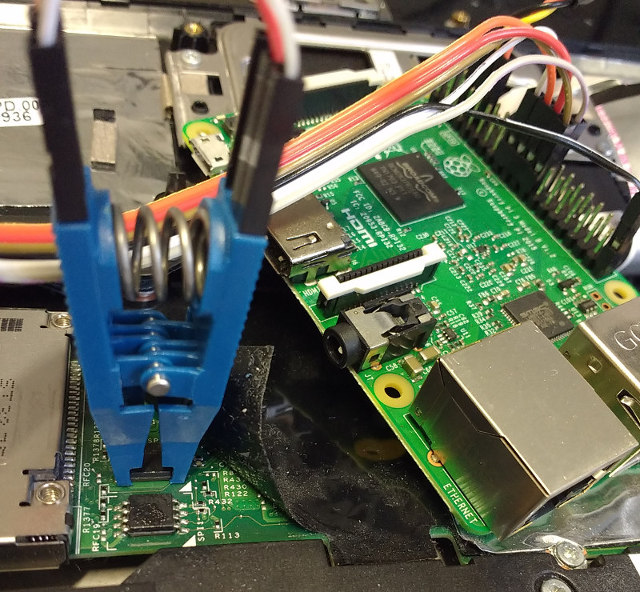
\includegraphics[width=0.5\textwidth]{rpi_clip.jpg}

\# ./external\_install\_top.sh -k "backup-file-to-create"

\# ./external\_install\_bottom.sh -m -k "backup-file-to-create"
\end{frame}


\begin{frame}
easy to use
\end{frame}


\begin{frame}

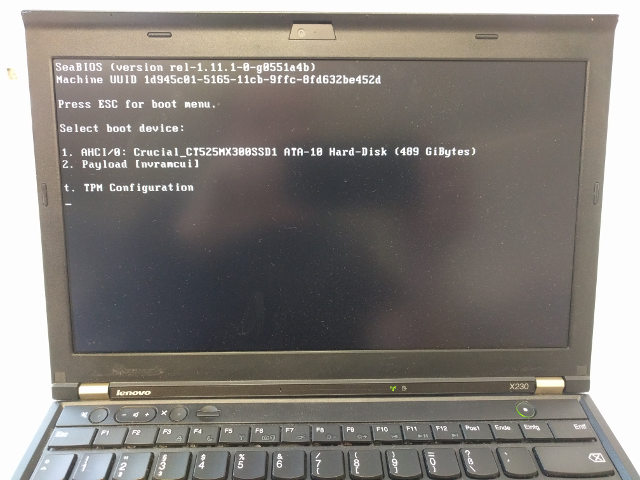
\includegraphics[width=\textwidth]{seabios}

\end{frame}


\begin{frame}
How does a release currently look like?
\end{frame}


\begin{frame}
Thinkpad X230 only. 2 different images:

- free software except microcode update binary

- Intel's proprietary VGABIOS (currently looks more beautiful)
\pause

coreboot master branch HEAD at time of release

latest SeaBIOS release

latest microcode update by Intel
\end{frame}


\begin{frame}
upstream work
\end{frame}


\begin{frame}
ensure latest SeaBIOS and MCU versions are in coreboot

test and update coreboot's board-status (Supported Motherboards wiki)
\end{frame}


\begin{frame}
recorded demo (there's not VGA/HDMI during reboot)
\end{frame}

\begin{frame}
https://github.org/merge/skulls

https://www.coreboot.org/users.html
\end{frame}

\end{document}
